%%%%%%%%%%%%%%%%%%%%%%%%%%%%%%%%%%%%%%%%%%%%%%%%%%%%%%%%%%%%%%%%%%%%%%%%%%%%%%%%
%neutrino_physics.tex: Chapter on neutrino physics:
%%%%%%%%%%%%%%%%%%%%%%%%%%%%%%%%%%%%%%%%%%%%%%%%%%%%%%%%%%%%%%%%%%%%%%%%%%%%%%%%
\chapter{Physics of Neutrinos}
\label{neutrino_physics_chapter}
%%%%%%%%%%%%%%%%%%%%%%%%%%%%%%%%%%%%%%%%%%%%%%%%%%%%%%%%%%%%%%%%%%%%%%%%%%%%%%%%

\section{Standard Model in a nutshell}
\begin{figure}
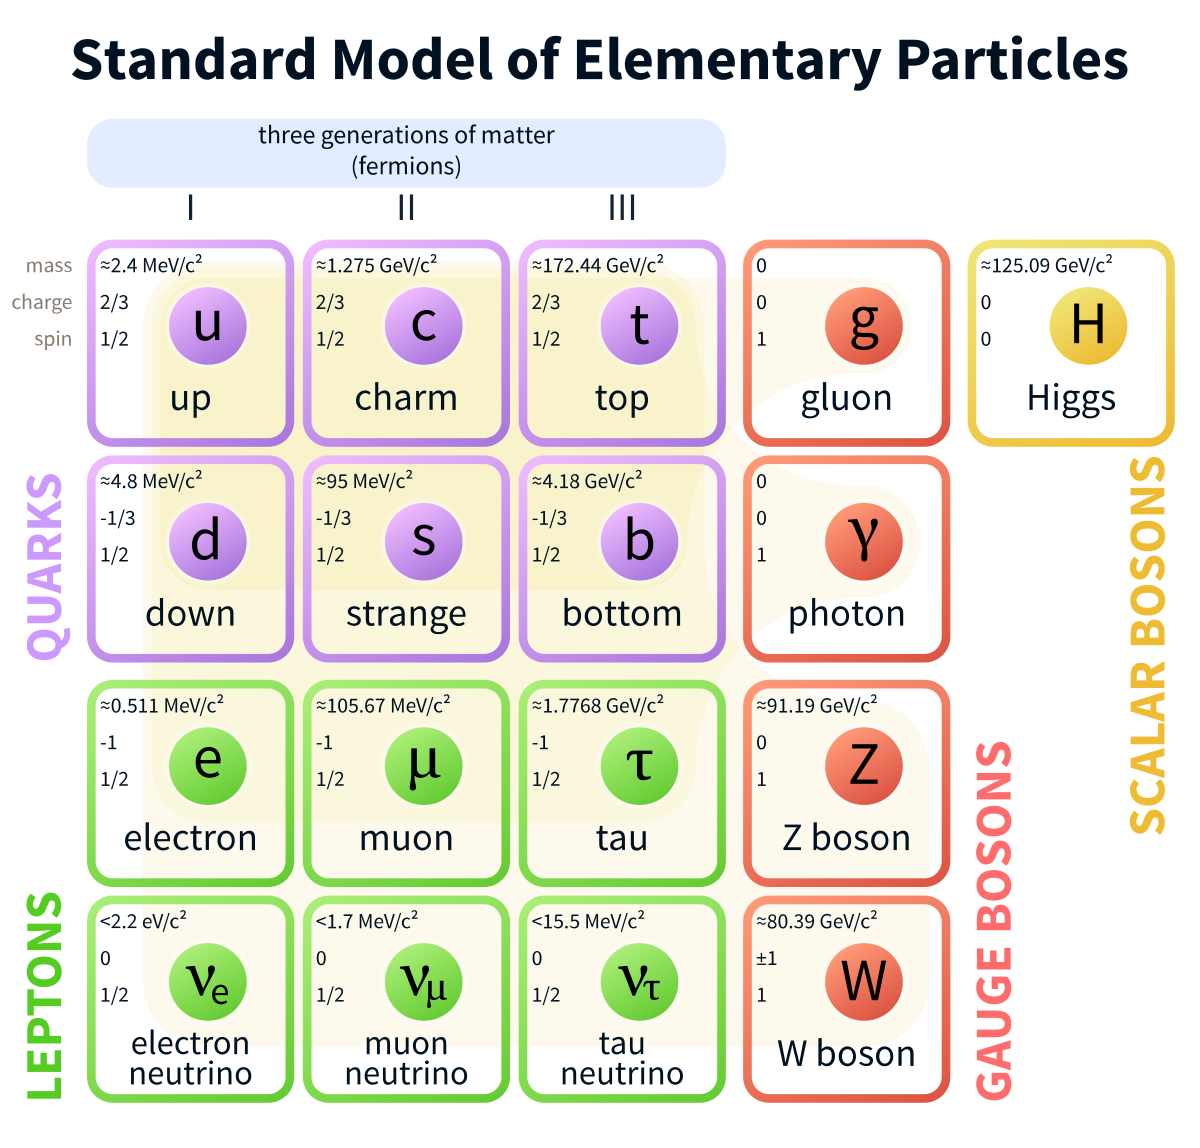
\includegraphics[width=0.8\textwidth]{figures/Standard_Model_of_Elementary_Particles.png}
\centering
\caption{Elementary Particles in the Standard Model.} \lb{SM}
\end{figure}
Since ancient times people were trying to understand the world around them. From 
first world models of ancient Greeks to modern theories scientists tried to use 
limited number of entities to decribe phenomena happened in nature - Democritus's 
indivisible atoms, Plato's elements (air, fire, water, earth) or elementary particles 
of the Standard Model. We do not have enough time to go over all theories but rather we 
concentrate on the latest and the most accurate one called Standard Model. 

Elementary particles of the Standrar Model are building blocks and glue of everything we
can see around us\footnote{As of today, Standard Model and Einstein's General Theory of 
Relativity could not fully explain motion of galaxies and exponential expansion of the Universe. 
Two more entities were introduced - dark matter for former phenomenon and dark energy 
for latter one.}. However, the most fascinating thing about the Model is that underlying 
principles which governs it are principles of symmetry, namely, gauge symmetry and Lorentz 
symmetry. The Standard Model's group is 
\be
SU(3)\times SU(2)\times U(1),
\ee 
where group $SU(3)$ describes strong interactions and $SU(2)\times U(1)$ describes 
electro-weak interactions\footnote{Gravitational interaction falls out of the picture
since for the last one hundred years gravity is described by deformation of space-time 
continium. Nevertheless, the attempts to rewrite gravity using the same language of groups
and unified it with Standard Model never were given up. In fact, all latest unified theories 
were based on groups of high demenstions where one of the most promising theories is 
String Theory.}. 

\section{Oscillations in Vacuum}
Neutrinos are massive elementary particles which participate in weak interactions 
and are immune to electromagnetic and strong interactions. They also participate 
in gravitational interactions, but since gravity is many orders of magnitude smaller 
in comparison to other forces one can neglect gravity effects completely, at least 
on energy scale of modern experiments. There are three types of neutrinos - 
with definite flavor - electron ($\nu_e$), muon ($\nu_\mu$) and tau ($\nu_\tau$) 
neutrinos. These flavor neutrinos are eigenstates of the weak Hamiltonian and they 
can be produced or destroyed only in weak interactions via exchange of the weak 
gauge bosons $W^\pm$ and $Z$. The neutrino mass eigenstates do not coincide with 
flavor eigenstates, and this leads to neutrino oscillations.

As was mentioned before flavor neutrinos are produced in weak interactions, but 
mass eigenstates are responsible for neutrino propagation through space. One can 
decompose the flavor eigenstates ($|\nu_e\rangle$, $|\nu_\mu\rangle$, $|\nu_\tau\rangle$) 
into linear combinations of mass eigenstates ($|\nu_1\rangle$, $|\nu_2\rangle$, $|\nu_3\rangle$).
\be
|\nu_f\rangle = \sum_{f=e,\mu,\tau}U_{fi}|\nu_i\rangle.
\ee
The matrix $U_{fi}$ is a $3\times 3$ unitary matrix and is called the lepton mixing matrix 
or PMNS (Pontecorvo, Maki, Nakagawa, Sakata) matrix. $U_{fi}$ encodes the neutrino 
mixing parameters such as $\theta_{12}$, $\theta_{13}$, $\theta_{23}$ and phase 
$\delta$ which is responsible for CP violation in weak interactions. The convenient 
parametrization is as follows:
\be
U_{fi} =
\left( \begin{array}{ccc}
c_{12}c_{13}                                & s_{12}c_{13}                                & s_{13}e^{-i\delta} \\
-s_{12}c_{23}-c_{12}s_{23}s_{13}e^{i\delta} & c_{12}c_{23}-s_{12}s_{23}s_{13}e^{i\delta}  & s_{23}c_{13} \\
s_{12}s_{23}-c_{12}c_{23}s_{13}e^{i\delta}  & -c_{12}s_{23}-s_{12}c_{23}s_{13}e^{i\delta} & c_{23}c_{13} \end{array} \right),
\ee
where $c_{ij} = \cos(\theta_{ij})$ and $s_{ij} = \sin(\theta_{ij})$.

Quantum mechanics governs how mass eigenstates propagate through space. Using the 
Schrodinger equation $-i\hbar\frac{\partial}{\partial t}|\psi\rangle = H|\psi\rangle$ 
one can derive a solution for neutrino wave function at the point $(x,t)$ of space-time 
starting with the wave function at the point $(0,0)$. Using the free Hamiltonian for 
neutrino mass eigenstates one derives \footnote{Natural units are used everywhere.}
\be
|\nu_i(x,t)\rangle = e^{-i(E_it - p_ix)}|\nu_i(0,0)\rangle.
\ee
Neutrino masses $m_i$ are much less in comparison neutrino energy in all experiments 
and the next ultra-relativistic approximation could be used
\be
p_i = \sqrt{E_i^2 - m_i^2} \approx E_i - \frac{m_i^2}{2E_i},
\ee
moreover, in this limit neutrino travels almost at the speed of light, so final solution 
for neutrino wave function with the mass $m_i$ is
\be
|\nu_i(L)\rangle = e^{-i\frac{m_i^2}{2E}L}|\nu_i(0)\rangle,
\ee
where $L$ is distance which the neutrino traveled.

If one creates a neutrino of flavor $f$ at $t=0$ and energy $E$ then the probability 
that at the distance $L$ from the neutrino source one observes a neutrino with flavor $f'$ is
\be
P_{\nu_f \rightarrow \nu_{f'}}(L, E) = |\langle\nu_{f}(0)|\nu_{f'} (L)\rangle|^2 \nn
\ee
\be
= \Big|\Big(\sum_{i}\langle\nu_{i}(0)|U_{fi}^*\Big)\Big(\sum_{i'}e^{-i\frac{m_{i'}^2}{2E}L}U_{f'i'}|\nu_{i'}(0)\rangle\Big)\Big|^2 \nn
\ee
\be
= \Big|\sum_i U_{fi}^*U_{f'i}e^{-i\frac{m_i^2}{2E}L}\Big|^2 \nn
\ee
\be
= \sum_{i=1}^3\sum_{j=1}^3 U_{fi}^*U_{f'i}U_{f'j}^*U_{fj}e^{-i\frac{\Delta m_{ij}^2}{2E}L},
\ee
where standard notation $\Delta m_{ij}^2 = m_i^2 - m_j^2$ was used. After a little bit of 
mathematics the last expression can be rewritten in the following form
\be
P_{\nu_f \rightarrow \nu_{f'}}(L, E) = \delta_{ff'}- 4\sum_{i>i'}\mathfrak{Re}(U_{fi}U_{fi'}^*U_{f'i'}^*U_{f'i})\sin^2\Big(\frac{\Delta m_{ij}^2}{4E}L\Big) +\nn
\ee
\be
+2\sum_{i>i'}\mathfrak{Im}(U_{fi}U_{fi'}^*U_{f'i'}^*U_{f'i})\sin\Big(\frac{\Delta m_{ij}^2}{2E}L\Big). \lb{Poscl}
\ee
It is worth noting that the oscillation probabilities depend on neutrino mass difference 
squared, therefore all neutrino oscillation experiments are sensitive only to $\Delta m_{ij}^2$. 
Also, in the case of a CP violation phase $\delta=0$ the last term in \p{Poscl} disappears 
and the oscillation probabilities are identical for neutrinos and antineutrinos. 
For the purpose of the experiment it is convenient to have the last equation when 
$\Delta m_{ij}$, $E$ and $L$ are expressed in $eV^2$, $GeV$ and $km$ respectively
\be
\frac{\Delta m_{ij}^2}{2E}L \quad\rightarrow\quad 1.27\frac{\Delta m_{ij}^2[eV^2]}{E[GeV]}L[km] = \Delta_{ij}.
\ee
The probabilities which are being measured by the NO$\nu$A experiment are the probabilities 
of muon neutrino disappearance and electron neutrino appearance
\be
P_{\nu_\mu \rightarrow \nu_\mu}(L, E) \approx 1 - \sin^2 2\theta_{23}\sin^2 \Delta_{32}, \lb{mu2mu}
\ee
\be
P_{\nu_\mu \rightarrow \nu_e}(L, E) \approx P_{atm} + P_{sol} + 2\sqrt{P_{atm}P_{sol}}(\cos\Delta_{32}\cos\delta \mp \sin\Delta_{32}\sin\delta), \lb{mu2e}
\ee
with
\be
P_{atm} = \sin^2\theta_{23}\sin^22\theta_{13}\sin^2\Delta_{31}, \qquad
P_{sol} \approx \cos^2\theta_{23}\cos^2\theta_{13}\sin^22\theta_{12}\Delta_{21}^2,
\ee
where the "-" sign in \p{mu2e} is for the neutrino and the "+" sign is for the anti-neutrino. 

\section{Oscillations in Matter}
%\begin{figure}
%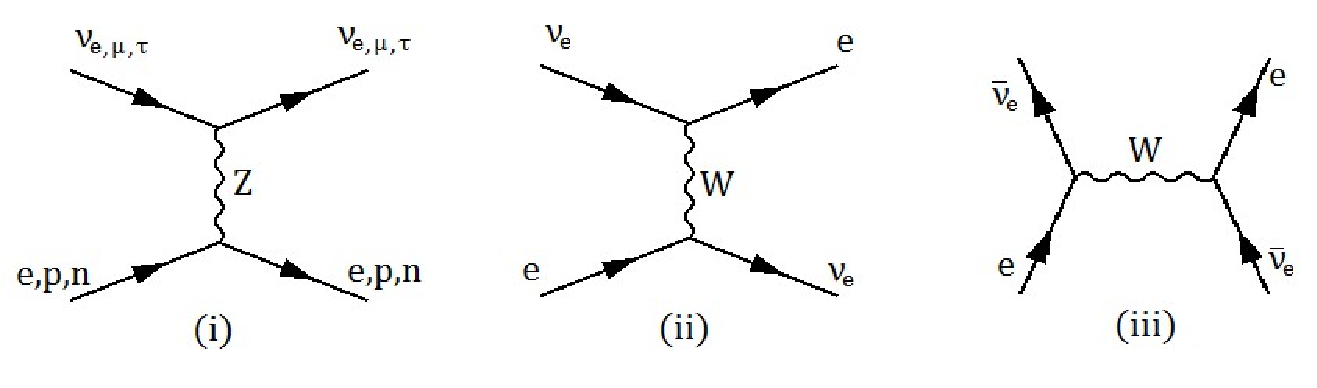
\includegraphics[width=0.9\textwidth]{NC_and_CC_currents.png}
%\centering
%\caption{Neutrino interaction with matter. (i) All neutrinos participate in NC interactions which leads to additional effective mass for all eigenstates $\nu_1, \nu_2$ and $\nu_3$, (ii) Additional CC interaction for electron neutrino $\nu_e$, which modifies mass square difference, (iii) effect similar to (ii) only for electron anti-neutrino $\bar{\nu}_e$. The diagram (iii) contributes with opposite sign in comparison to (ii).} \lb{NC}
%\end{figure}

Each neutrino studied by the NO$\nu$A experiment travels through the Earth's crust for more 
than 810 km. While propagating through matter, neutrinos interact with medium constituting 
particles which leads to changes in neutrino oscillations. Since interaction going through 
exchange of only weak gauge bosons there are two types of possible interaction: (i) neutrino 
emits $Z$ boson - neutral current (NC) interaction and (ii) neutrino emits $W^\pm$ boson - 
charged current (CC) interaction. In matter all three flavors of neutrinos interact through 
exchange $Z$ boson with electrons, protons and neutrons. But only for electron neutrino there 
is another possibility - interaction through exchange $W^+$ boson with electrons as can be 
seen in the figure \p{NC}.

Accounting for interactions between neutrinos and all matter found on Earth adds two additional 
terms to the Hamiltonian which describes neutrino propagation - effective potential,
\be
V_{C} = \sqrt{2}G_{F}N_e \qquad and \qquad V_{N} = -\frac{1}{\sqrt{2}}G_{F}N_n,
\ee
where $G_F$ is Fermi constant, $N_e$ and $N_n$ electron and neutron number density respectively. 
The second term effectively shifts all $m_i^2 \rightarrow m_i^2 + 2|\mathbf{p}|V_N$ and does not 
have an effect on $\Delta m_{ij}$. The first term $V_C$ enters the Hamiltonian in a such way 
that it has an influence only on the electron neutrino $\nu_e$, and has the opposite influence 
on electron anti-neutrino $\bar{\nu}_e$. After further calculations one can derive the following 
corrected expressions for $\Delta m_{32}$ and $\sin 2\theta_{13}$ in the presence of matter
\be
\Delta m_{32}^2\Big|_{mat} = \sqrt{(\Delta m_{32}^2 \sin2\theta_{13})^2 + (\Delta m_{32}^2\cos2\theta_{13} \mp 2E_\nu V_C)^2} \nn
\ee
\be
\sin 2\theta_{13}\Big|_{mat} = \frac{\Delta m_{32}^2 \sin 2\theta_{13}}{\sqrt{(\Delta m_{32}^2 \sin2\theta_{13})^2 + (\Delta m_{32}^2\cos2\theta_{13} \mp 2E_\nu V_C)^2}}
\ee
The matter effect has a significant influence on $\nu_e$ appearance probability and in the first approximation
\be
P_{\nu_\mu \rightarrow \nu_e}(E,L)\Big|_{mat} = \Big(1 \pm \frac{2E_\nu V_C}{\Delta m_{32}^2}\Big)P_{\nu_\mu \rightarrow \nu_e}(E,L),
\ee
where the "+" sign is for the neutrino and the "-" sign is for the antineutrino. This effect 
is known as the Mikheyev-Smirnov-Wolfenstein (MSW) effect, and for the NO$\nu$A experiment it 
plays an important role in helping to determine the CP violating phase $\delta_{CP}$.
%\begin{figure}
%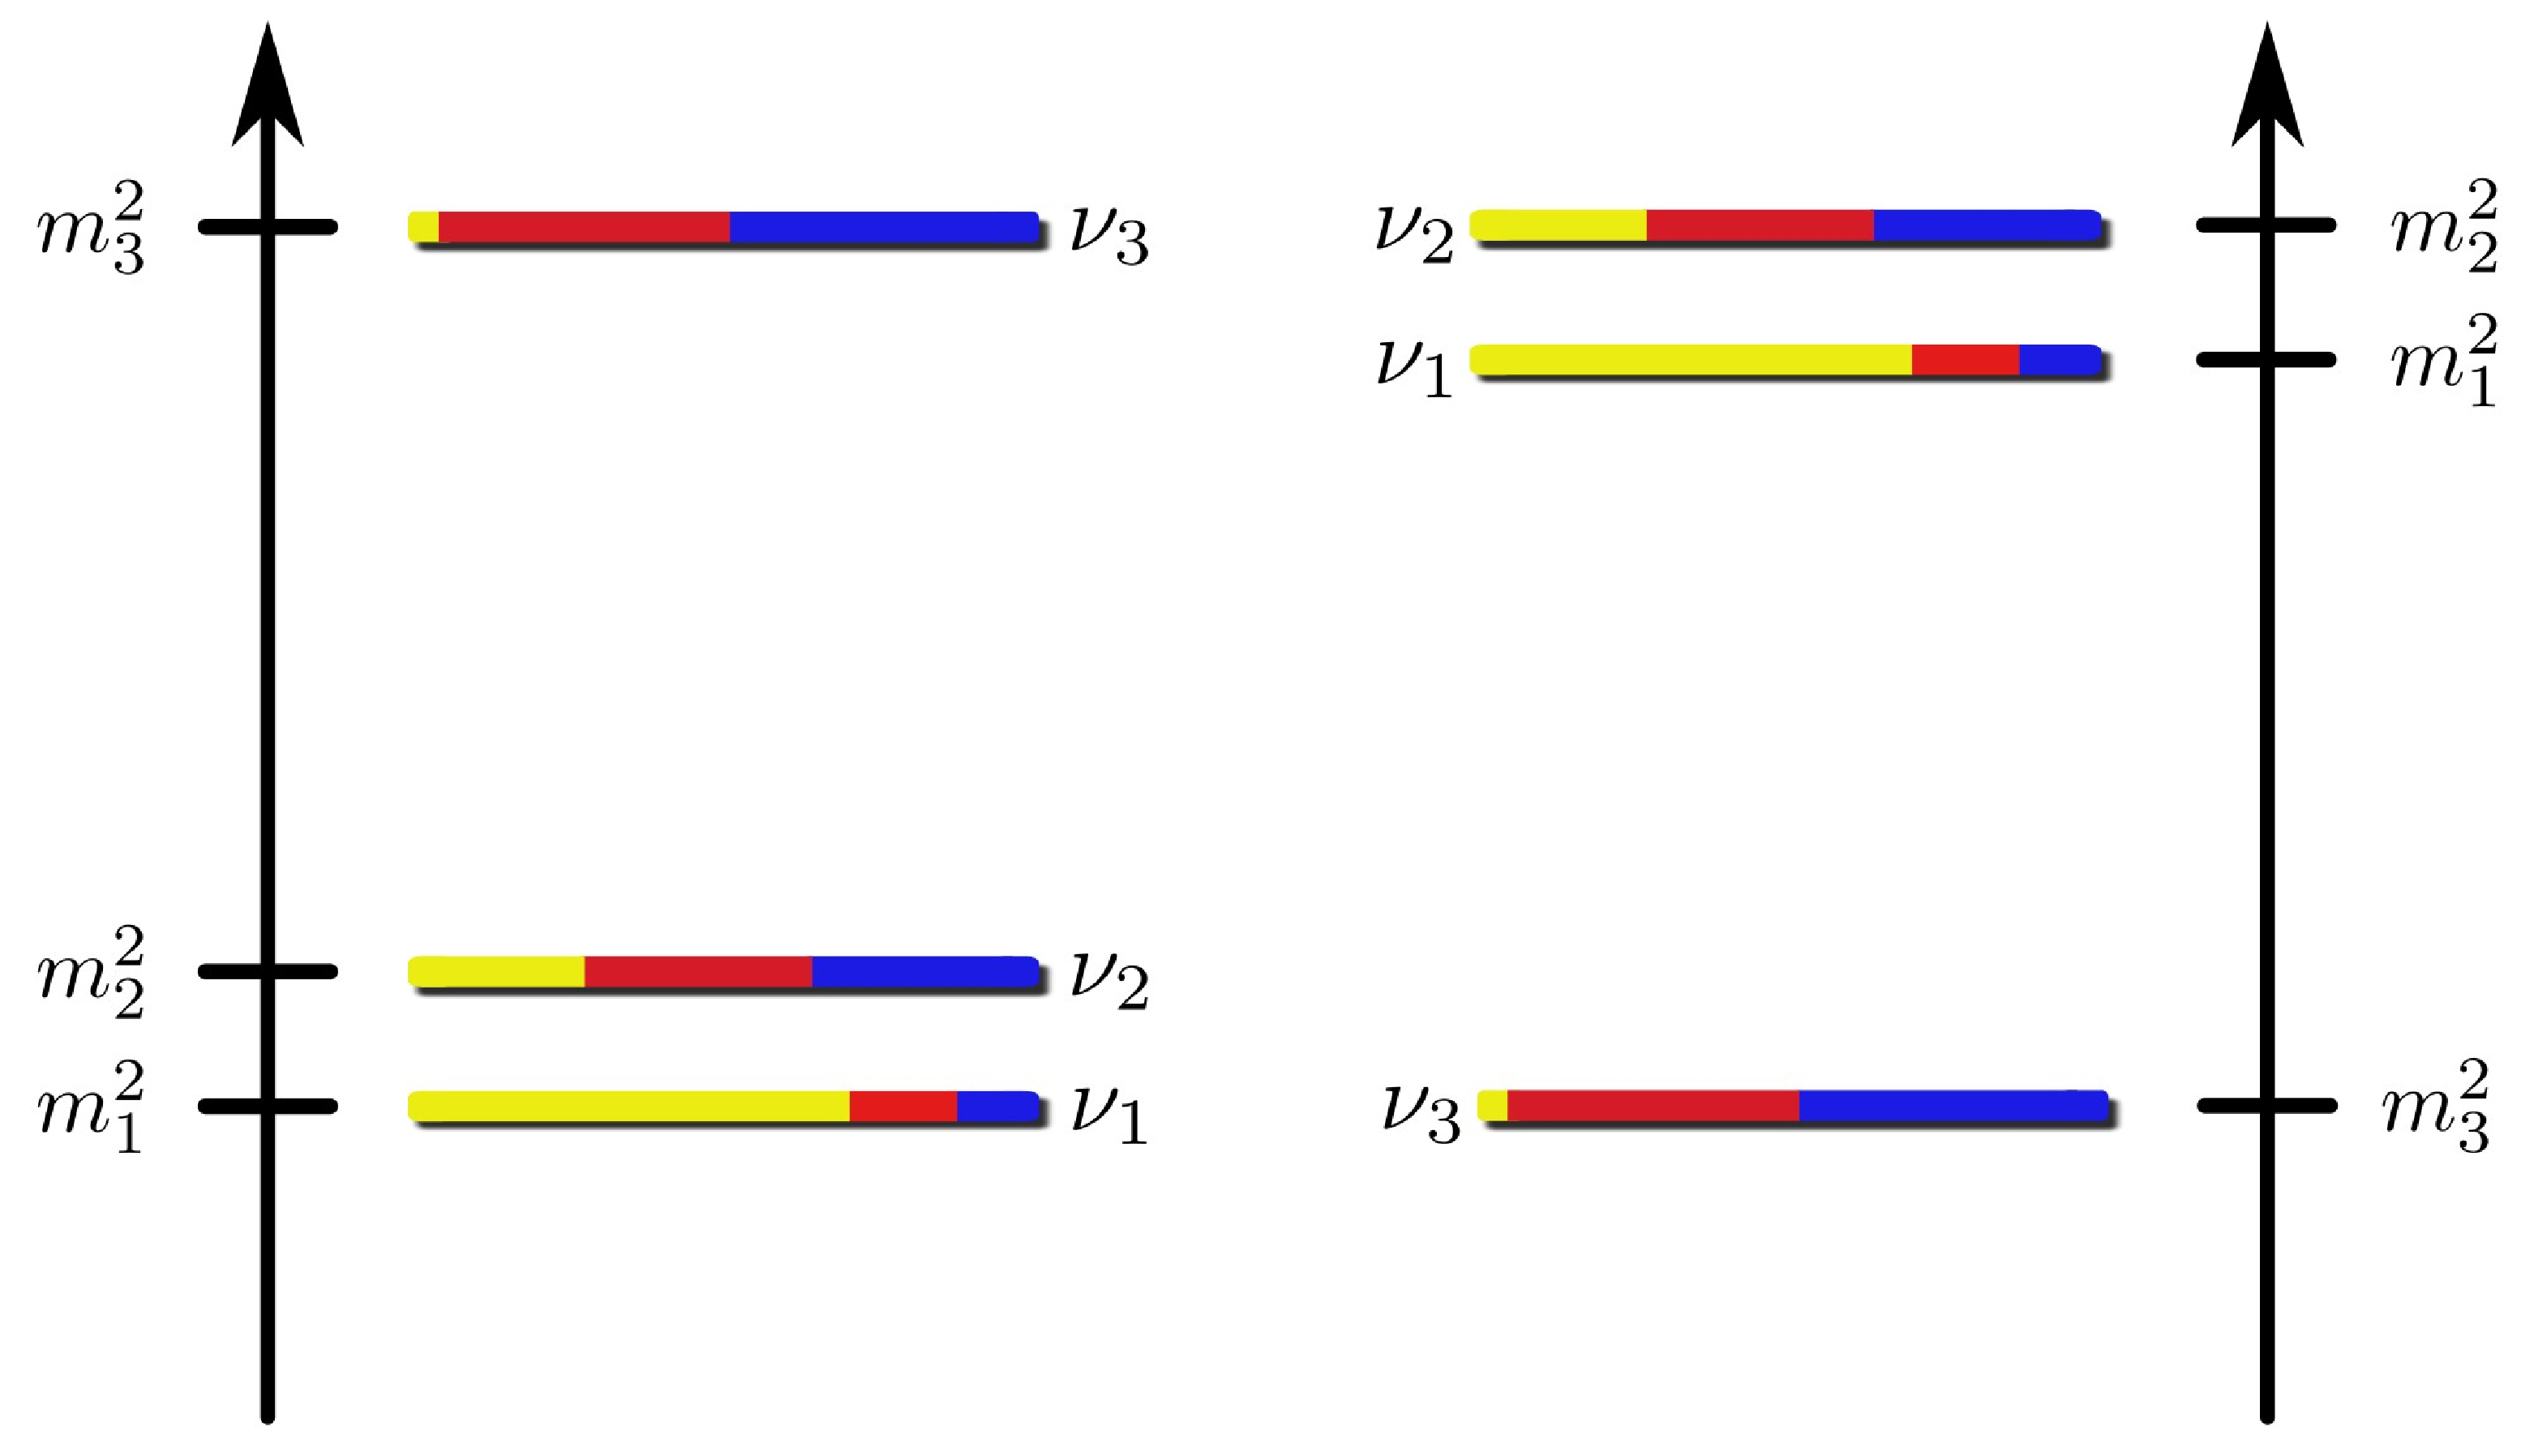
\includegraphics[width=0.8\textwidth]{Nu_hierarchy.png}
%\centering
%\caption{Two possible variants of neutrino mass hierarchies. The left side corresponds to the normal hierarchy (NH) and right side corresponds to the inverted hierarchy (IH). Colors represent how much and what kind of neutrino flavors contribute to every mass state. The electron flavor is yellow, muon flavor is red and the tau flavor is blue.} \label{NH}
%\end{figure}

It is worth noting that assigning specific masses to specific mass states are completely 
arbitrary, but it is known from experimental data that two masses are much closer to each other 
in comparison with the third mass. These two masses are called $m_1$ and $m_2$, with $m_2 > m_1$ 
and $\Delta m_{12} << |\Delta m_{32}| \approx |\Delta m_{31}|$. However, the sign of $\Delta m_{32}$ 
is still unknown. That leaves two possibilities which are called normal hierarchy (NH) and inverted 
hierarchy (IH). Figure \p{NH} illustrates the neutrino mass distributions. The NO$\nu$A experiment 
will be able to determine which hierarchy is realized in nature.

%%%%%%%%%%%%%%%%%%%%%%%%%%%%%%%%%%%%%%%%%%%%%%%%%%%%%%%%%%%%%%%%%%%%%%%%%%%%%%%%

%%%%%%%%%%%%%%%%%%%%%%%%%%%%%%%%%%%%%%%%%%%%%%%%%%%%%%%%%%%%%%%%%%%%%%%%%%%%%%%%
